\documentclass[zavrsnirad]{fer}
% Dodaj opciju upload za generiranje konačne verzije koja se učitava na FERWeb
% Add the option upload to generate the final version which is uploaded to FERWeb


\usepackage{blindtext}
\usepackage{listings}
\usepackage{color, colortbl}
\usepackage{tabularx}

\usepackage{graphicx}
\usepackage{amsmath}

\definecolor{codebg}{rgb}{0.95, 0.95, 0.95}
\lstset{
	backgroundcolor=\color{codebg},
	basicstyle=\footnotesize\ttfamily,
	frame=single,
	rulecolor=\color{black},
	numbers=left,
	numberstyle=\tiny\color{gray},
	keywordstyle=\color{blue},
	commentstyle=\color{green},
	stringstyle=\color{red},
	breaklines=true,
	captionpos=b,
	escapeinside={(*@}{@*)}
}



%--- PODACI O RADU / THESIS INFORMATION ----------------------------------------

% Naslov na engleskom jeziku / Title in English
\title{Machine Learning Model for Alzheimer's Disease Classification Using Brain MRI Images}

% Naslov na hrvatskom jeziku / Title in Croatian
\naslov{Model strojnog učenja za klasifikaciju Alzheimerove bolesti uporabom slika magnetske rezonancije mozga}

% Broj rada / Thesis number
\brojrada{1291}

% Autor / Author
\author{Petra Buršić}

% Mentor 
\mentor{Doc.dr.sc\@ Jelena Božek}

% Datum rada na engleskom jeziku / Date in English
\date{June, 2024}

% Datum rada na hrvatskom jeziku / Date in Croatian
\datum{lipanj, 2024.}

%-------------------------------------------------------------------------------


\begin{document}


% Naslovnica se automatski generira / Titlepage is automatically generated
\maketitle


%--- ZADATAK / THESIS ASSIGNMENT -----------------------------------------------

% Zadatak se ubacuje iz vanjske datoteke / Thesis assignment is included from external file
% Upiši ime PDF datoteke preuzete s FERWeb-a / Enter the filename of the PDF downloaded from FERWeb
\zadatak{zadatak.pdf}


%--- ZAHVALE / ACKNOWLEDGMENT --------------------------------------------------

\begin{zahvale}
  % Ovdje upišite zahvale / Write in the acknowledgment
  Hvala mentorici i obitelji za podršku kroz rad.
\end{zahvale}


% Sadržaj se automatski generira / Table of contents is automatically generated
\tableofcontents


% Odovud započinje numeriranje stranica / Page numbering starts from here
\mainmatter


%--- UVOD / INTRODUCTION -------------------------------------------------------
\chapter{Uvod}
\label{pog:uvod}

Alzheimerova bolest (AD) predstavlja jedan od najvećih medicinskih i društvenih izazova suvremenog doba. Prema podacima Svjetske zdravstvene organizacije, AD je vodeći uzrok demencije, stanja koje trenutno pogađa preko 50 milijuna ljudi širom svijeta, a predviđa se da će se taj broj udvostručiti svakih 20 godina, dosežući 152 milijuna do 2050. godine \cite{PMID:29763097}. U Hrvatskoj, gdje oko 16\% populacije čine osobe starije od 65 godina, procjenjuje se da oko 80,000 ljudi pati od demencije, od čega većinu čine pacijenti s Alzheimerovom bolesti \cite{MIMICA2010409}. Ova bolest karakterizira progresivni gubitak kognitivnih funkcija, što značajno narušava svakodnevni život pojedinca i njegovih skrbnika. Rana dijagnoza AD-a može značajno pomoći u upravljanju simptomima i planiranju skrbi, ali trenutno ne postoji pouzdani lijek koji bolest može izliječiti ili znatno usporiti njezin napredak \cite{PMID:29763097}.
\\
Demencija, kao rezultat AD-a, uzrokuje značajne promjene u mozgu. Jedna od glavnih karakteristika je nakupljanje beta-amiloidnih plakova izvan neurona i neurofibrilarnih čvorova unutar neurona \cite{10.1007/s00500-020-05292-x}. Oni dovode do smrti moždanih stanica i gubitka sinaptičke veze između neurona. Kao posljedica toga, dolazi do atrofije mozga, posebno u područjima koja su ključna za pamćenje, kao što je hipokampus, te u korteksu koji je odgovoran za mišljenje, planiranje i pamćenje \cite{doi:10.1212/WNL.0b013e3181c3f293}.
\\
MRI (Magnetic Resonance Imaging), posebno strukturni MRI, je neinvazivna tehnika snimanja koja pruža detaljne slike anatomije mozga. Široko se koristi za otkrivanje strukturnih promjena u mozgu povezanih s AD-om, kao što su atrofija hipokampusa i promjene u kortikalnoj debljini \cite{10.3389/fnins.2015.00307}. 
\\
Strojno učenje pruža moćne alate za analizu velikih skupova podataka i može značajno unaprijediti sposobnost dijagnoze složenih bolesti poput AD-a. Algoritmi strojnog učenja mogu analizirati obrasce u MRI slikama i prepoznati suptilne promjene koje možda nisu odmah vidljive stručnjacima, čime se povećava točnost i učinkovitost dijagnoze.
\\
Uz pomoć strukturnih MRI slika iz baze podataka Alzheimer’s Disease Neuroimaging Initiative (ADNI), u ovom radu primijenit ćemo dvije metode strojnog učenja, Stablo odluke (DT) i Support Vector Machine (SVM), kako bismo razvili, testirali i usporedili modele sposobne za klasifikaciju pojedinaca u tri kategorije: zdrave osobe (CN), osobe s blagim kognitivnim oštećenjem (MCI) i osobe s Alzheimerovom bolešću (AD).


%-------------------------------------------------------------------------------
\label{pog:glavni_dio}

\chapter{Magnetska rezonancija}

Magnetska rezonancija (MRI) je neinvazivna tehnika snimanja koja koristi magnetska polja i radiovalove za stvaranje detaljnih slika unutarnjih struktura tijela. Konvencionalna MRI se široko koristi za radiološku dijagnozu i stvara prostorne mape svojstava mobilnih vodikovih jezgri (protona) koje se uglavnom nalaze u molekulama vode. Kontrast unutar slika proizlazi iz varijacija u gustoći vode unutar tkiva i načinu na koji voda reagira s makromolekulama \cite{Gore2003}. Postoje tri glavne vrste MRI-a: strukturni MRI (sMRI), funkcionalni MRI (fMRI) i difuzijski MRI (dMRI).


\section{Strukturni MRI (sMRI)}
Strukturni MRI je ključan za diferencijalnu dijagnozu Alzheimerove bolesti zbog svoje sposobnosti vizualizacije specifičnih obrazaca atrofije u mozgu. T1-mjerene slike, koje se često koriste u strukturnom MRI-u, imaju visoku kontrastnu rezoluciju između sive i bijele tvari, što omogućuje precizno razlikovanje ovih tkiva i identifikaciju atrofičnih promjena povezanih s AD-om \cite{Gonuguntla2022}. Siva tvar sadrži većinu neuronskih tijela, dok bijela tvar sadrži mijelinizirane aksonske puteve koji povezuju različite dijelove sive tvari. T1-mjerene slike prikazuju masno tkivo i mijelin kao svijetle, dok tekućine poput cerebrospinalne tekućine izgledaju tamno (Slika \ref{fig:sMRI_T1}).

\begin{figure}[h]
	\centering
	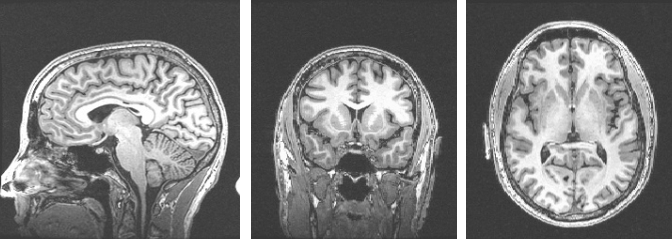
\includegraphics[width=1\textwidth]{Figures/T1_sMRI.png}
	\caption{T1 sMRI slika \cite{ucsd2021}}
	\label{fig:sMRI_T1}
\end{figure}

 U ovom radu koristimo strukturne MRI slike iz ADNI baze podataka kako bismo razvili, testirali i usporedili modele strojnog učenja za klasifikaciju Alzheimerove bolesti. Korištenje strukturnih MRI podataka omogućuje precizno identificiranje regija mozga koje su zahvaćene AD-om, što je ključno za razumijevanje progresije bolesti i razvoj učinkovitih metoda za njezinu dijagnozu i praćenje \cite{Gonuguntla2022}.


\section{Funkcionalni MRI (fMRI)}

Funkcionalni MRI (fMRI) koristi se za detekciju malih promjena u signalima koji se koriste za proizvodnju MR slika koje su povezane s neuronskom aktivnošću u mozgu (Slika \ref{fig:fMRI}). 

fMRI detektira promjene ovisne o razini kisika u krvi (BOLD, Blood-Oxygen-Level Dependent) koje se javljaju kada se promjene u neuronskoj aktivnosti dogode nakon promjene stanja mozga, poput stimulusa ili zadatka. Ova tehnika je sigurna, neinvazivna i ponovljiva kod odraslih i djece, te ima široke potencijalne primjene u osnovnoj i kliničkoj neuroznanosti \cite{Gore2003}. Na slici \ref{fig:fMRI_BOLD} prikazana je promjena BOLD signala u odnosu na neuronsku aktivnost, ilustrirajući kako fMRI detektira metaboličke promjene povezane s neuronskom aktivnošću.


\begin{figure}[h]
	\centering
	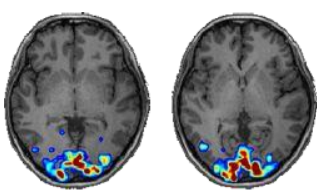
\includegraphics[width=0.5\textwidth]{Figures/fMRI.png}
	\caption{fMRI slika \cite{ucsd2021}}
	\label{fig:fMRI}
\end{figure}

\begin{figure}[h]
	\centering
	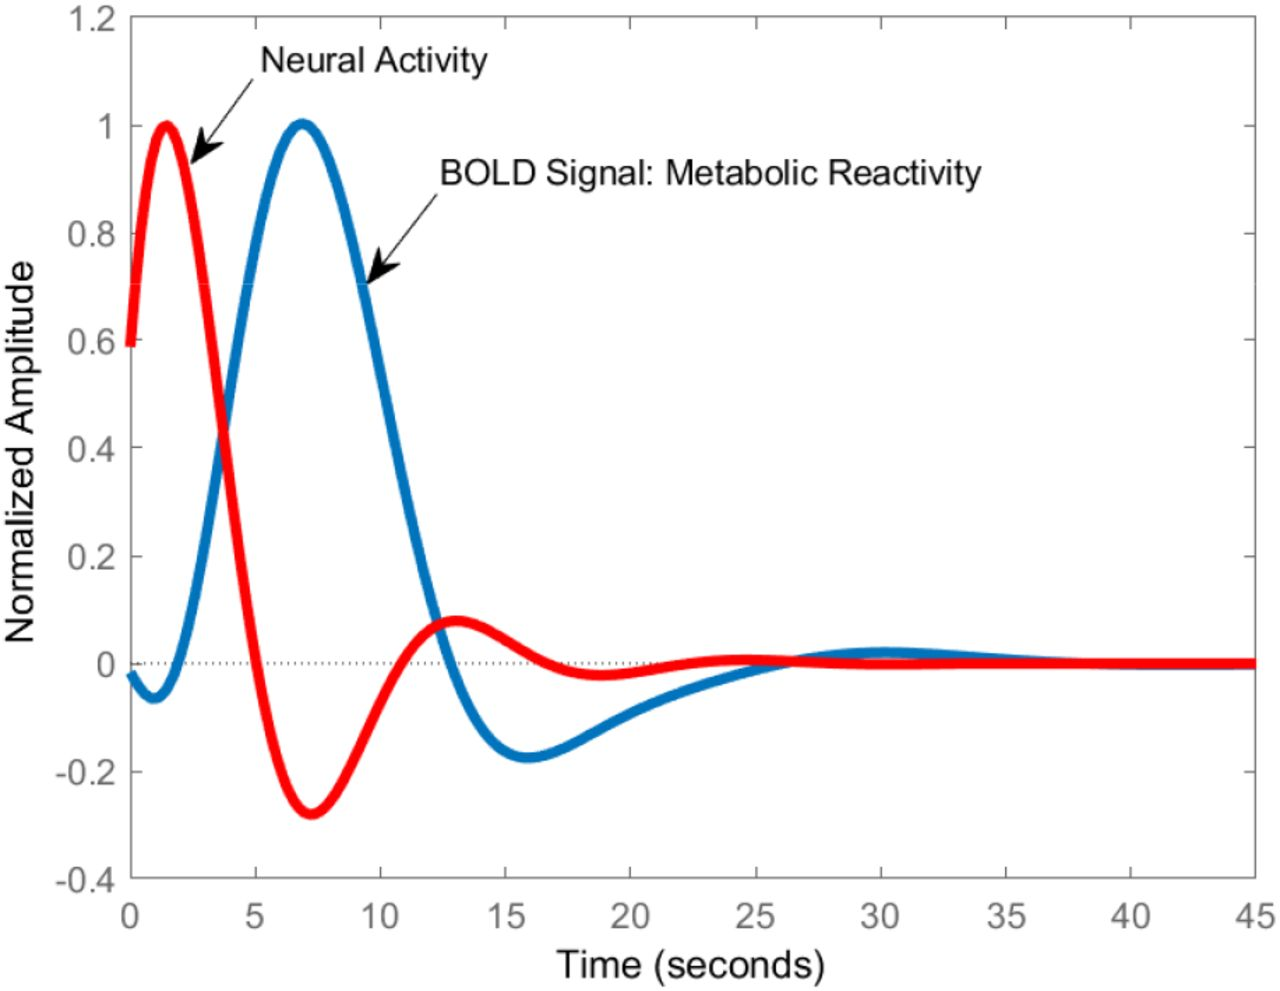
\includegraphics[width=0.7\textwidth]{Figures/BOLD.jpg}
	\caption{Promjena BOLD (Blood-Oxygen-Level Dependent) signala u odnosu na neuronsku aktivnost.\cite{Schaper573006}}
	\label{fig:fMRI_BOLD}
\end{figure}


\section{Difuzijski MRI (dMRI)}
Difuzijski MRI (dMRI) koristi se za mjerenje difuzije molekula vode u tkivima, što može pružiti informacije o mikrostrukturi mozga. dMRI tehnika može otkriti mikroskopske promjene u tkivima u ranim fazama AD-a, poput gubitka mijelina, oštećenja aksona i gubitka neurona \cite{Promteangtrong2015}.

Jedna od najčešće korištenih metoda u dMRI je difuzijska tenzorska slika (DTI) \ref{fig:dMRI}, koja omogućuje kvantifikaciju smjera i veličine difuzije vode, pružajući detaljne informacije o integritetu bijele tvari u mozgu. Cilj većine dMRI studija je usporediti DTI metrike između dviju ili više populacija ispitanika ili istražiti korelacije između DTI metrika i relevantnih kognitivnih mjera \cite{mueller2015diffusion}.

\begin{figure}[h]
	\centering
	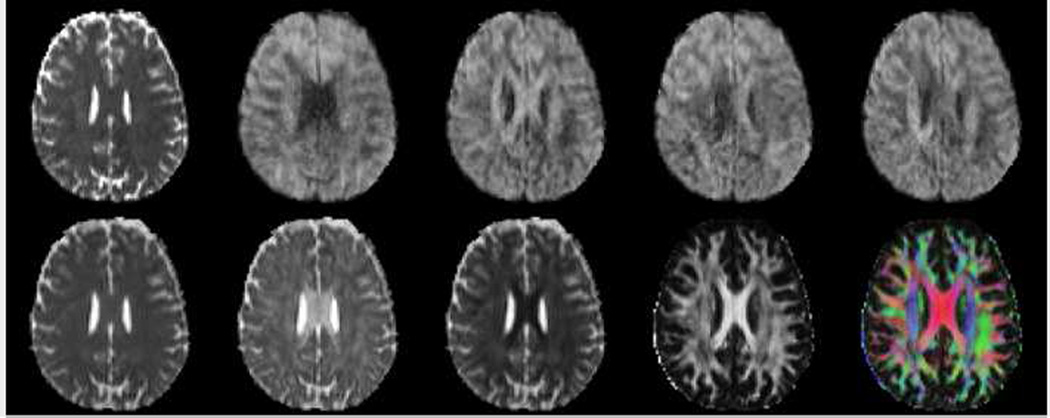
\includegraphics[width=0.7\textwidth]{Figures/dMRI.jpg}
	\caption{Primjer DTI podataka zdravog ispitanika \cite{mueller2015diffusion}}
	\label{fig:dMRI}
\end{figure}


\chapter{Strojno učenje (ML)}
Strojno učenje (ML) je grana umjetne inteligencije koja se temelji na razvijanju algoritama koji mogu učiti iz podataka i donositi odluke na temelju naučenih obrazaca \cite{ml_book}. Strojno učenje se dijeli na tri vrste: nadzirano učenje, nenadzirano učenje i učenje pojačanjem.

\section{Vrste strojnog učenja}

\subsection{Nadzirano učenje}

Nadzirano učenje uključuje treniranje modela na označenom skupu podataka, što znači da je svaki primjer učenja uparen s izlaznom oznakom. Cilj je da model nauči mapirati ulaze na ispravan izlaz.

Uobičajeni algoritmi uključuju:

\begin{itemize}
	\item \textbf{Stablo odluke}: Algoritmi koji koriste strukturu stabla za donošenje odluka i predikciju rezultata na temelju ulaznih podataka \cite{somvanshi2016}.
	\item \textbf{Support Vector Machines (SVM)}: Algoritmi koji analiziraju podatke za klasifikaciju i regresiju, koristeći hiperplane za razdvajanje različitih klasa \cite{somvanshi2016}.
	\item \textbf{K najbližih susjeda (k-Nearest Neighbors)}: Algoritam koji klasificira podatke na temelju sličnosti s najbližim susjedima u skupu podataka \cite{mahesh2019}.
	\item \textbf{Random Forest}: Ansambl algoritama koji koristi više stabala odlučivanja za poboljšanje točnosti i smanjenje pretreniranosti \cite{mahesh2019}.
\end{itemize}

\subsection{Nenadzirano učenje}

Nenadzirano učenje bavi se podacima koji nemaju označene odgovore. Sustav pokušava naučiti obrasce i strukture iz podataka.

Ključne metode uključuju:

\begin{itemize}
	\item \textbf{Klasteriranje}: Algoritmi poput K-meansa koji dijele skup podataka u klastere na temelju sličnosti značajki \cite{somvanshi2016}.
	\item \textbf{Analiza glavnih komponenata (PCA)}: Tehnika koja se koristi za smanjenje dimenzionalnosti podataka pretvaranjem u novi skup varijabli koje su nekorelirane i koje hvataju maksimalnu varijabilnost \cite{somvanshi2016}.
\end{itemize}

\subsection{Učenje pojačanjem}

Učenje pojačanjem odnosi se na učenje najboljih akcija koje treba poduzeti u nekom okruženju kako bi se maksimizirala kumulativna nagrada. Uključuje agenta koji interaktivno djeluje s okruženjem i uči postići cilj isprobavajući različite akcije i primajući povratne informacije u obliku nagrada ili kazni \cite{mahesh2019}.

\subsection{Ključni koncepti i primjene}

\begin{itemize}
	\item \textbf{Odabir i ekstrakcija značajki}: Ključno u predprocesiranju podataka za modele strojnog učenja. Cilj je odabrati relevantne značajke koje poboljšavaju performanse modela.
	\item \textbf{Evaluacija modela}: Metode poput unakrsne validacije koriste se za procjenu performansi modela strojnog učenja i sprječavanje overfittinga \cite{ibm_machine_learning}.
	\item \textbf{Primjene}: Strojno učenje koristi se u raznim aplikacijama kao što su prepoznavanje slika i govora, medicinska dijagnostika, financije (npr. kreditno bodovanje i algoritamsko trgovanje) i personalizirane preporuke \cite{ibm_machine_learning}.
\end{itemize}


\section{Stablo odluke}
Stablo odluke (DT, Decision Tree) je model strojnog učenja koji koristi različite značajke ekstrahirane iz MRI slika kako bi predvidio prisutnost ili odsutnost Alzheimerove bolesti. DT pruža intuitivan i vizualno razumljiv način predstavljanja odluka temeljenih na ovim značajkama, omogućujući jednostavno tumačenje i analizu klasifikacijskih pravila \cite{somvanshi2016}.

Stablo odluke je tehnika temeljena na stablu u kojoj je svaki put koji započinje od korijena opisan nizom za razdvajanje podataka sve dok se ne postigne finalni ishod u listu čvora \cite{Charbuty_Abdulazeez_2021}. Ovo omogućuje modelu da jasno i precizno identificira različite kategorije na temelju danih podataka.

\subsection{Primjer stabla odluke}
Na slici \ref{fig:decision_tree} prikazan je primjer stabla odluke koje može biti korišteno za klasifikaciju na temelju različitih atributa. Svaki čvor u stablu testira određeni atribut kao što su "Temperatura", "Kiša" ili "Sunce", dok grane predstavljaju različite vrijednosti tih atributa koje vode do konačnih klasifikacija kao što su "Pulover", "Kišobran" ili "Majica".

\begin{figure}[h]
	\centering
	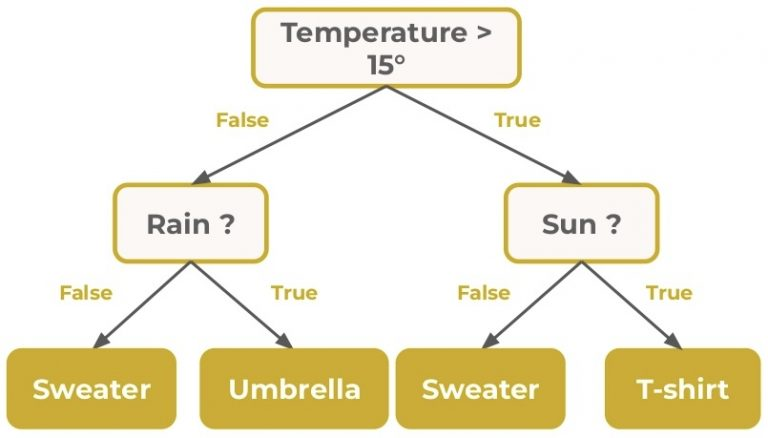
\includegraphics[width=0.6\textwidth]{Figures/DecisionTree.jpg}
	\caption{Primjer stabla odlučivanja \cite{Keldenich2022}}
	\label{fig:decision_tree}
\end{figure}

\subsection{Algoritmi stabla odluke}
Postoji nekoliko algoritama za izgradnju stabala odluke, a najpoznatiji među njima su ID3, C4.5 i CART.

\subsubsection{ID3 (Iterative Dichotomiser 3)}
ID3 algoritam je vrlo jednostavan algoritam za izgradnju stabla odlučivanja koji je razvio Quinlan 1986. godine. Ovaj algoritam koristi kriterij informacijske dobiti za odabir atributa na svakom čvoru stabla, što maksimizira smanjenje entropije. Prednosti uključuju brzo građenje stabla i stvaranje razumljivih pravila, dok nedostaci uključuju osjetljivost na numeričke atribute i nedostatak rukovanja s nedostajućim vrijednostima \cite{singh2014}.

\subsubsection{C4.5}
C4.5 je evolucija ID3 algoritma, također razvijenog od strane Quinlana. Ovaj algoritam koristi omjer dobiti kao kriterij za odabir atributa i omogućuje rukovanje kontinuiranim i diskretnim atributima, kao i nedostajućim vrijednostima. C4.5 također koristi strategiju rezanja stabala kako bi se smanjila prekomjerna prilagodba \cite{singh2014}.

\subsubsection{CART (Classification and Regression Trees)}
CART, koji su razvili Breiman i suradnici, koristi binarno grananje i Towing kriterij za odabir podjela. Ovaj algoritam može generirati klasifikacijska i regresijska stabla te omogućuje rukovanje numeričkim i kategoričkim podacima. CART također koristi strategiju rezanja stabala za smanjenje složenosti stabla \cite{singh2014}.


\subsection{Prednosti i nedostaci}
Stabla odlučivanja nude nekoliko prednosti:
\begin{itemize}
	\item Jednostavna za razumijevanje i interpretaciju.
	\item Zahtijevaju malo predobrade podataka.
	\item Mogu rukovati numeričkim i kategoričkim podacima.
	\item Sposobna su za rukovanje nedostajućim vrijednostima.
\end{itemize}

Međutim, imaju i neke nedostatke:
\begin{itemize}
	\item Sklona su prekomjernom prilagođavanju, posebno kod složenih stabala.
	\item Mogu biti nestabilna; male promjene u podacima mogu dovesti do različitih struktura stabla.
	\item Sklona su pristranosti prema atributima s više razina \cite{Charbuty_Abdulazeez_2021}\cite{somvanshi2016}.
\end{itemize}



\section{Slučajna šuma}
Slučajna šuma (RF, Random forest) je jedan od najmoćnijih i najpopularnijih algoritama strojnog učenja. Razvio ga je Leo Breiman 2001. godine kao ansambl metodu koja koristi mnoštvo stabala odlučivanja kako bi poboljšala točnost i stabilnost modela. Slučajna šuma može se koristiti za klasifikaciju i regresiju, a poznat je po svojoj otpornosti na prekomjerno prilagođavanje.

Slučajna šuma sastoji se od velikog broja individualnih stabala odlučivanja koja djeluju kao ansambl. Svako stablo u šumi daje klasifikaciju (za klasifikacijske probleme) ili predviđanje (za regresijske probleme), a glasanje ili prosjek tih rezultata određuje konačni ishod modela. Ključni koncepti Random Forest algoritma uključuju bootstrap uzorkovanje, slučajni odabir podskupa značajki za svaki čvor stabla, i agregaciju rezultata pomoću glasanja ili prosjeka \cite{geeksforgeeks2021}.

\subsection{Koraci algoritma RF}
Slika \ref{fig:random_forest} prikazuje postupak algoritma RF za klasifikaciju.
\begin{itemize} 
	\item Model Treniranje: više odluka stabala se trenira koristeći različite podskupove podataka za trening.
	\item Model Testiranje: Svako stablo daje svoju predikciju, a konačna odluka se donosi većinskim glasanjem (bagging) tih predikcija.
\end{itemize}

\begin{figure}[h]
	\centering
	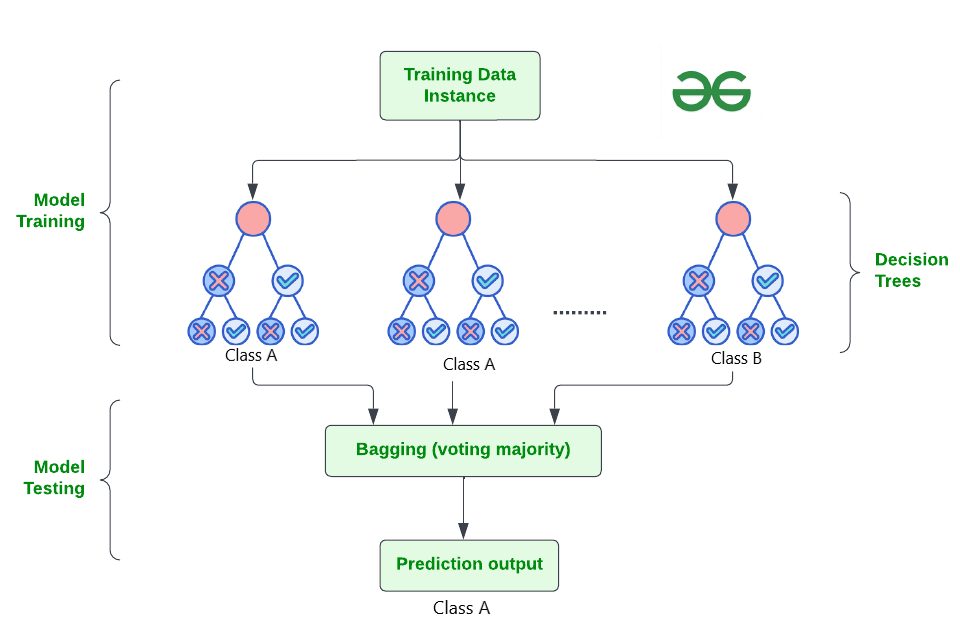
\includegraphics[width=0.8\textwidth]{Figures/random_forests.png}
	\caption{Izgradnja Random Forest algoritma \cite{geeksforgeeks2021}}
	\label{fig:random_forest}
\end{figure}

\subsubsection{Bootstrap uzorkovanje}
Svako stablo u Random Forest-u trenira se na drugačijem bootstrap uzorku podataka. To znači da se za svako stablo nasumično odabire podskup podataka s ponavljanjem iz originalnog skupa podataka, što rezultira različitim uzorcima za svako stablo. Ovaj pristup smanjuje varijancu modela i povećava njegovu otpornost na prekomjerno prilagođavanje \cite{segal2004machine}.

\subsubsection{Slučajni odabir značajki}
Za svaki čvor u stablu odlučivanja, Random Forest nasumično odabire podskup značajki iz cijelog skupa značajki i koristi ih za određivanje najboljeg razdvajanja. Ovaj postupak dodatno smanjuje korelaciju među stablima u šumi i poboljšava ukupnu točnost modela \cite{segal2004machine}.

\subsubsection{Agregacija rezultata}
Nakon što se sva stabla u šumi treniraju, rezultati svake klasifikacije ili predikcije agregiraju se kako bi se dobio konačni rezultat. Za klasifikacijske probleme koristi se većinsko glasanje, dok se za regresijske probleme koristi prosjek svih predikcija \cite{sarica2017}.

\subsubsection{Prednosti RF algoritma}
RF ima nekoliko ključnih prednosti:
\begin{itemize}
	\item Otpornost na prekomjerno prilagođavanje: Korištenje više stabala smanjuje rizik od prekomjernog prilagođavanja modela na trenirajući skup podataka.
	\item Rad s velikim brojem značajki: Slučajni odabir podskupa značajki omogućuje modelu da učinkovito radi s velikim brojem značajki.
	\item Stabilnost: RF je stabilniji u prisutnosti šuma i outliera u podacima.
	\item Intrinzična selekcija značajki: Model prirodno pruža mjere važnosti značajki koje mogu pomoći u razumijevanju podataka i njihovom utjecaju na predikcije \cite{sarica2017}.
\end{itemize}


\section{Stroj potpornih vektora (SVM)}
Stroj potpornih vektora je algoritam strojnog učenja koji koristi koncept marginizacije kako bi klasificirao podatke. Osnovna ideja SVM-a je pronaći hiperravninu koja najbolje razdvaja podatke u različite klase. Ključni koncepti SVM-a uključuju odvajajuću hiperravninu, hiperravninu s maksimalnom marginom, mekanu marginu i kernel funkciju \cite{fletcher2009}.

\subsection{Odvajajuća hiperravnina}
Odvajajuća hiperravnina je pravac ili ravnina koja razdvaja skup podataka u dvije klase \ref{fig:odv_hiper}. U dvodimenzionalnom prostoru, ovo je jednostavna linija, dok je u višedimenzionalnom prostoru to hiperravnina \cite{Noble2006}.
\begin{figure}[h]
	\centering
	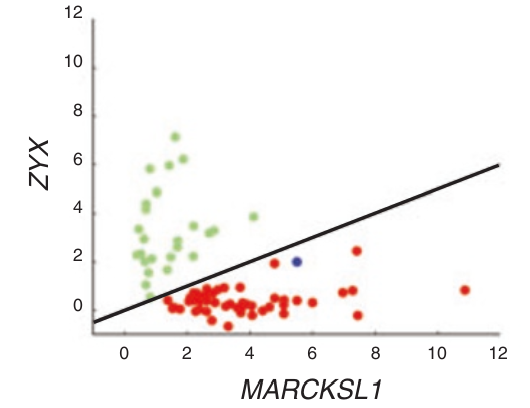
\includegraphics[width=0.6\textwidth]{Figures/odv_hiperravnina.png}
	\caption{Odvajajuća hiperravnina. \cite{Noble2006}}
	\label{fig:odv_hiper}
\end{figure}

\subsection{Hiperravnina s maksimalnom marginom}
Hiperravnina s maksimalnom marginom je ona koja maksimalno povećava udaljenost između najbližih točaka (potpornih vektora) iz svake klase \ref{fig:maks_marg}. Ova metoda osigurava da je klasifikacija što točnija i generaliziranija na nove podatke \cite{Noble2006}.
\begin{figure}[h]
	\centering
	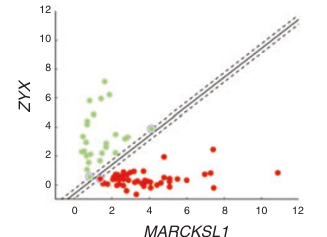
\includegraphics[width=0.6\textwidth]{Figures/maks_margina.png}
	\caption{Hiperravnina s maksimalnom marginom. Potporni vektori su zaokruženi. \cite{Noble2006}}
	\label{fig:maks_marg}
\end{figure}

\subsection{Hiperravnina s mekanom marginom}
Za podatke koji nisu savršeno razdvojivi, SVM koristi koncept mekane margine koja dopušta neke pogreške klasifikacije. Ovaj pristup uvodi varijable kazni kako bi uravnotežio broj pogrešno klasificiranih primjera i širinu margine \cite{fletcher2009}.
\begin{figure}[h]
	\centering
	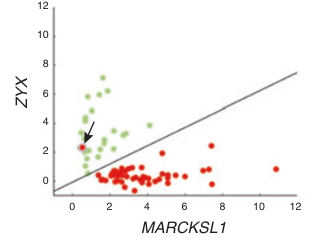
\includegraphics[width=0.6\textwidth]{Figures/soft_margin.png}
	\caption{Hiperravnina s mekanom marginom. Strelica pokazuje na pogrešku. \cite{Noble2006}}
	\label{fig:soft_margin}
\end{figure}

\subsection{Kernel funkcija}
Kernel funkcija omogućuje SVM-u da rješava nelinearno odvojive podatke tako što mapira ulazne podatke u višedimenzionalni prostor gdje postaju linearno odvojivi. Popularne kernel funkcije uključuju polinomijalne, radijalne bazne funkcije (RBF) i sigmoidne kernele \cite{Gammermann2000}.

\subsection{Primjene SVM-a}
SVM algoritmi imaju širok raspon primjena, od prepoznavanja obrazaca i regresije do biomedicinskih klasifikacija poput automatske klasifikacije mikroarray ekspresijskih profila gena \cite{Noble2006}.

\chapter{Podaci i metode}
\section{ADNI baza podataka}
Alzheimer's Disease Neuroimaging Initiative (ADNI) je studija pokrenuta 2004. godine s ciljem razvoja kliničkih, slikovnih, genetičkih i biokemijskih biomarkera za rano otkrivanje i praćenje Alzheimerove bolesti. ADNI uključuje sudionike u dobi od 55 do 90 godina koji su regrutirani na više od 50 lokacija u Sjedinjenim Američkim Državama i Kanadi \cite{adni_about}. 

ADNI baza podataka prikuplja širok spektar podataka koji uključuju slike mozga (MRI i PET), genetske podatke, kognitivne testove, kao i biomarkere iz cerebrospinalne tekućine i krvi \cite{adni_about}. Ovi podaci omogućuju istraživačima proučavanje odnosa između kliničkih, kognitivnih, slikovnih, genetičkih i biokemijskih karakteristika AD-a tijekom evolucije bolesti.

Sudionici u ADNI studiji podijeljeni su u nekoliko skupina:

\begin{itemize}
	\item \textbf{Normalni kontrolni sudionici (CN)}: Osobe bez znakova depresije, blagih kognitivnih oštećenja ili demencije.
	\item\textbf{Sudionici s blagim kognitivnim oštećenjem (MCI)}: Osobe koje pokazuju blage kognitivne deficite, ali ne zadovoljavaju kriterije za dijagnozu demencije.
	\item \textbf{Sudionici s Alzheimerovom bolešću (AD)}: Osobe s dijagnozom blage Alzheimerove bolesti.
\end{itemize}

Glavni ciljevi ADNI-a uključuju \cite{adni_about}:
\begin{itemize}
	\item Praćenje longitudinalnih promjena u kogniciji i biomarkerima.
	\item Predikcija kognitivnog pada.
	\item Validacija biomarkera.
	\item Optimizacija dizajna kliničkih ispitivanja.
	\item Otkriće novih genetskih i proteinskih markera povezanih s AD-om.
\end{itemize}

Podaci prikupljeni iz ADNI baze podataka dostupni su istraživačima putem LONI Image and Data Archive (IDA) \cite{usc_loni}, gdje mogu pristupiti slikama, kliničkim, genomskim i biomarkernim podacima za znanstvena istraživanja, podučavanje ili planiranje kliničkih studija.

\section{Analiza korištenih podataka}
Za potrebe istraživanja korišteni su podaci iz Alzheimer's Disease Neuroimaging Initiative (ADNI) baze podataka. Konkretno, korištene su visokokvalitetne strukturne MRI pretprocesirane slike snimljene na 3T uređaju, koje su preuzete u .NIfTI formatu \ref{fig:nifti}.

\begin{figure}[h]
	\centering
	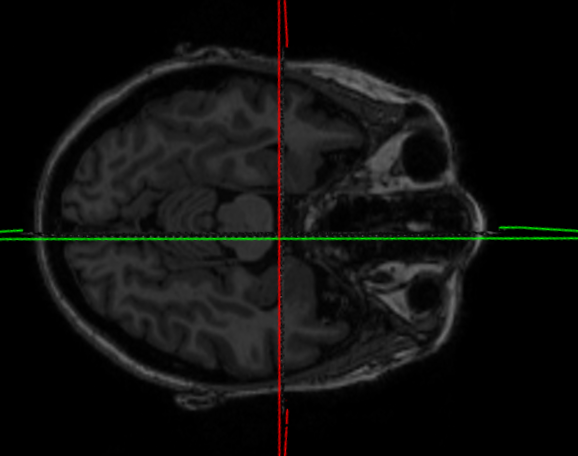
\includegraphics[width=0.5\textwidth]{Figures/primjer_slike.png}
	\caption{sMRI slika NIfTi formata prikazana u BrainVieweru\cite{umich_brainviewer}}
	\label{fig:nifti}
\end{figure}


Skup podataka korišten u ovom istraživanju sastoji se od informacija o sudionicima iz različitih dijagnostičkih grupa: AD (Alzheimerova bolest), CN (kontrolna skupina) i MCI (blagi kognitivni poremećaj). Svaki zapis sadrži podatke o \textbf{identifikacijskom broju slike, subjektu, grupi, spolu, dobi, posjeti, modalitetu i opisu MRI snimka}.

Ukupan broj sudionika u istraživanju je \textbf{148}. Raspodjelu sudionika u tri dijagnostičke grupe možemo vidjeti u Tablici \ref{tab:brojsudionikapogrupi}.

\begin{table}[ht]
	\centering
	\begin{tabular}{|c|c|}
		\hline
		\textbf{Grupa} & \textbf{Broj sudionika} \\
		\hline
		AD & 33 \\
		CN & 47 \\
		MCI & 68 \\
		\hline
	\end{tabular}
	\caption{Broj sudionika po grupi}
	\label{tab:brojsudionikapogrupi}
\end{table}

Sudionici su raspodijeljeni po spolu kako slijedi: muškaraca (M) je 73, dok je žena (F) 75. Ova distribucija prikazana je u Tablici \ref{tab:raspodjelaspol}.

\begin{table}[ht]
	\centering
	\begin{tabular}{|c|c|c|}
		\hline
		\textbf{Grupa} & \textbf{Muškarci} & \textbf{Žene} \\
		\hline
		AD & 11 & 22 \\
		CN & 18 & 29 \\
		MCI & 44 & 24 \\
		\hline
	\end{tabular}
	\caption{Raspodjela sudionika po grupi i spolu}
	\label{tab:raspodjelaspol}
\end{table}

Kako bismo se nosili s neravnotežom u klasama unutar skupa podataka, koristili smo tehniku \textbf{prekomjernog uzorkovanja }(oversampling). Oversampling tehnika umjetno generira dodatne uzorke za klase s manjim brojem podataka, čime se postiže bolja uravnoteženost dataset-a. To omogućuje modelima da bolje uče iz podataka i smanjuje pristranost prema većim klasama, poboljšavajući ukupnu učinkovitost klasifikacije. 

\begin{figure}[h]
	\centering
	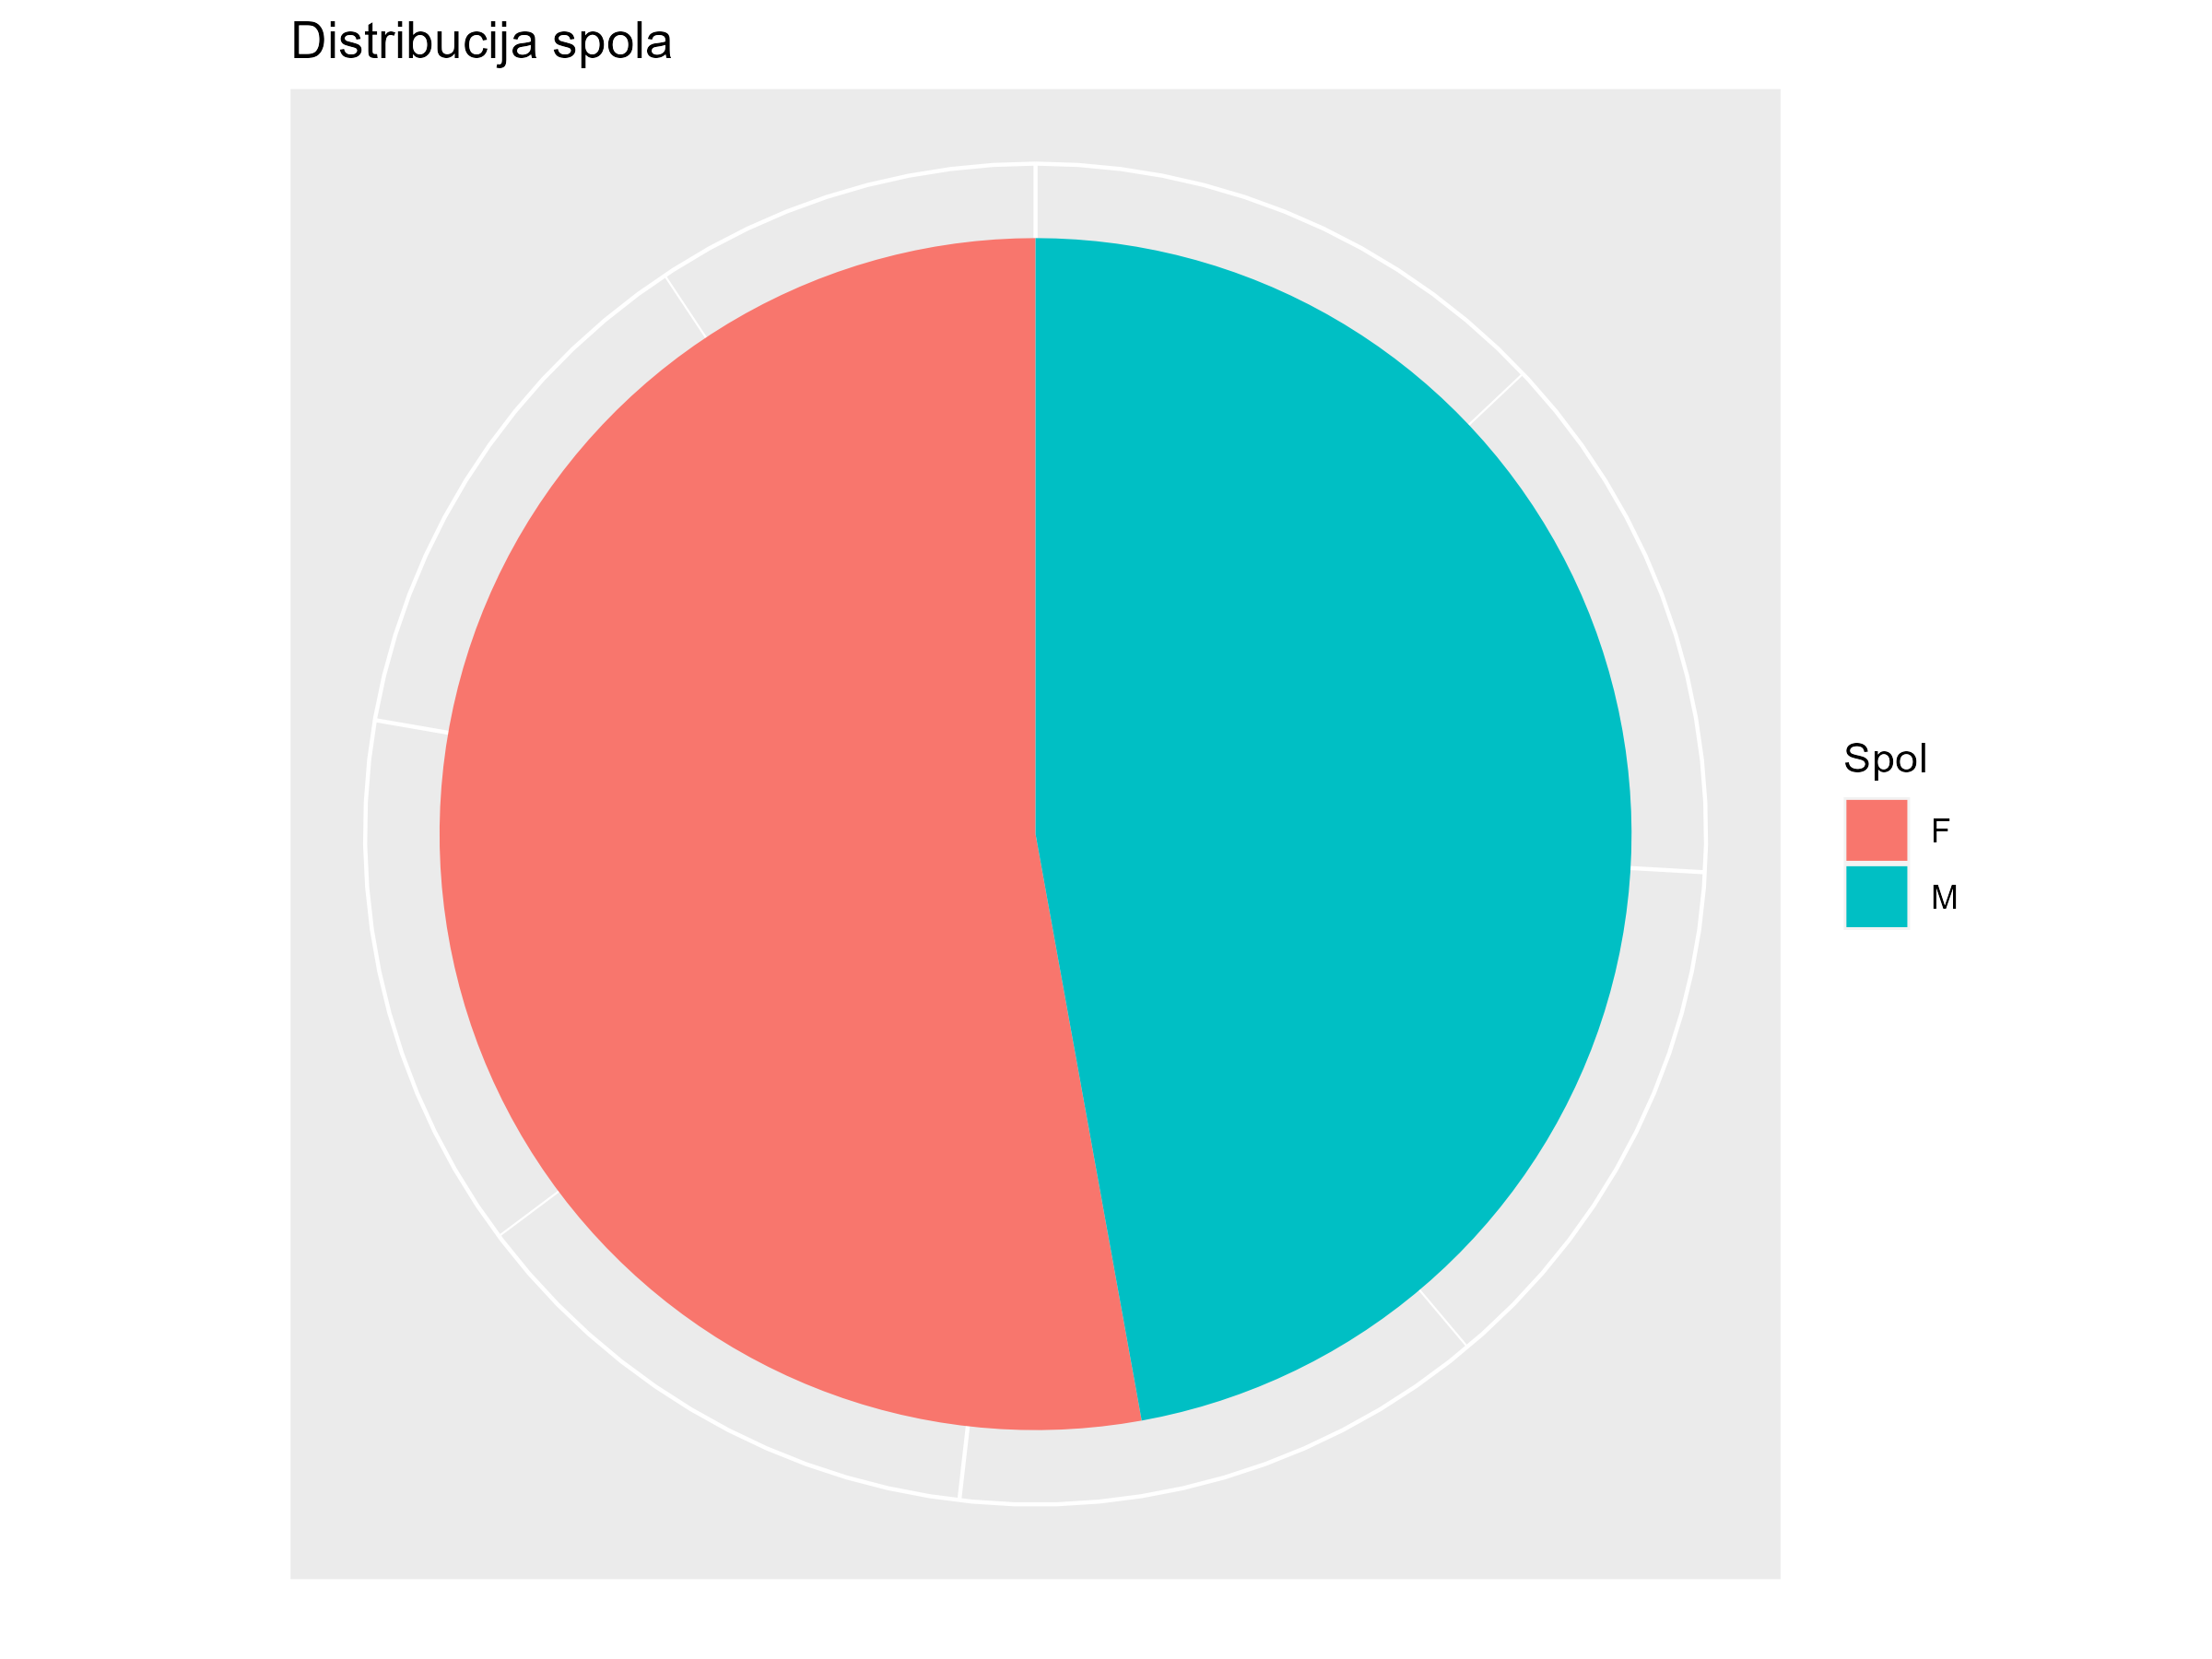
\includegraphics[width=0.6\textwidth]{Figures/pie_chart_spola.png}
	\caption{Raspodjela sudionika po spolu}
	\label{fig:spol}
\end{figure}

Dobnu raspodjelu sudionika možemo vidjeti na slici \ref{fig:dob}.
\begin{figure}[h]
	\centering
	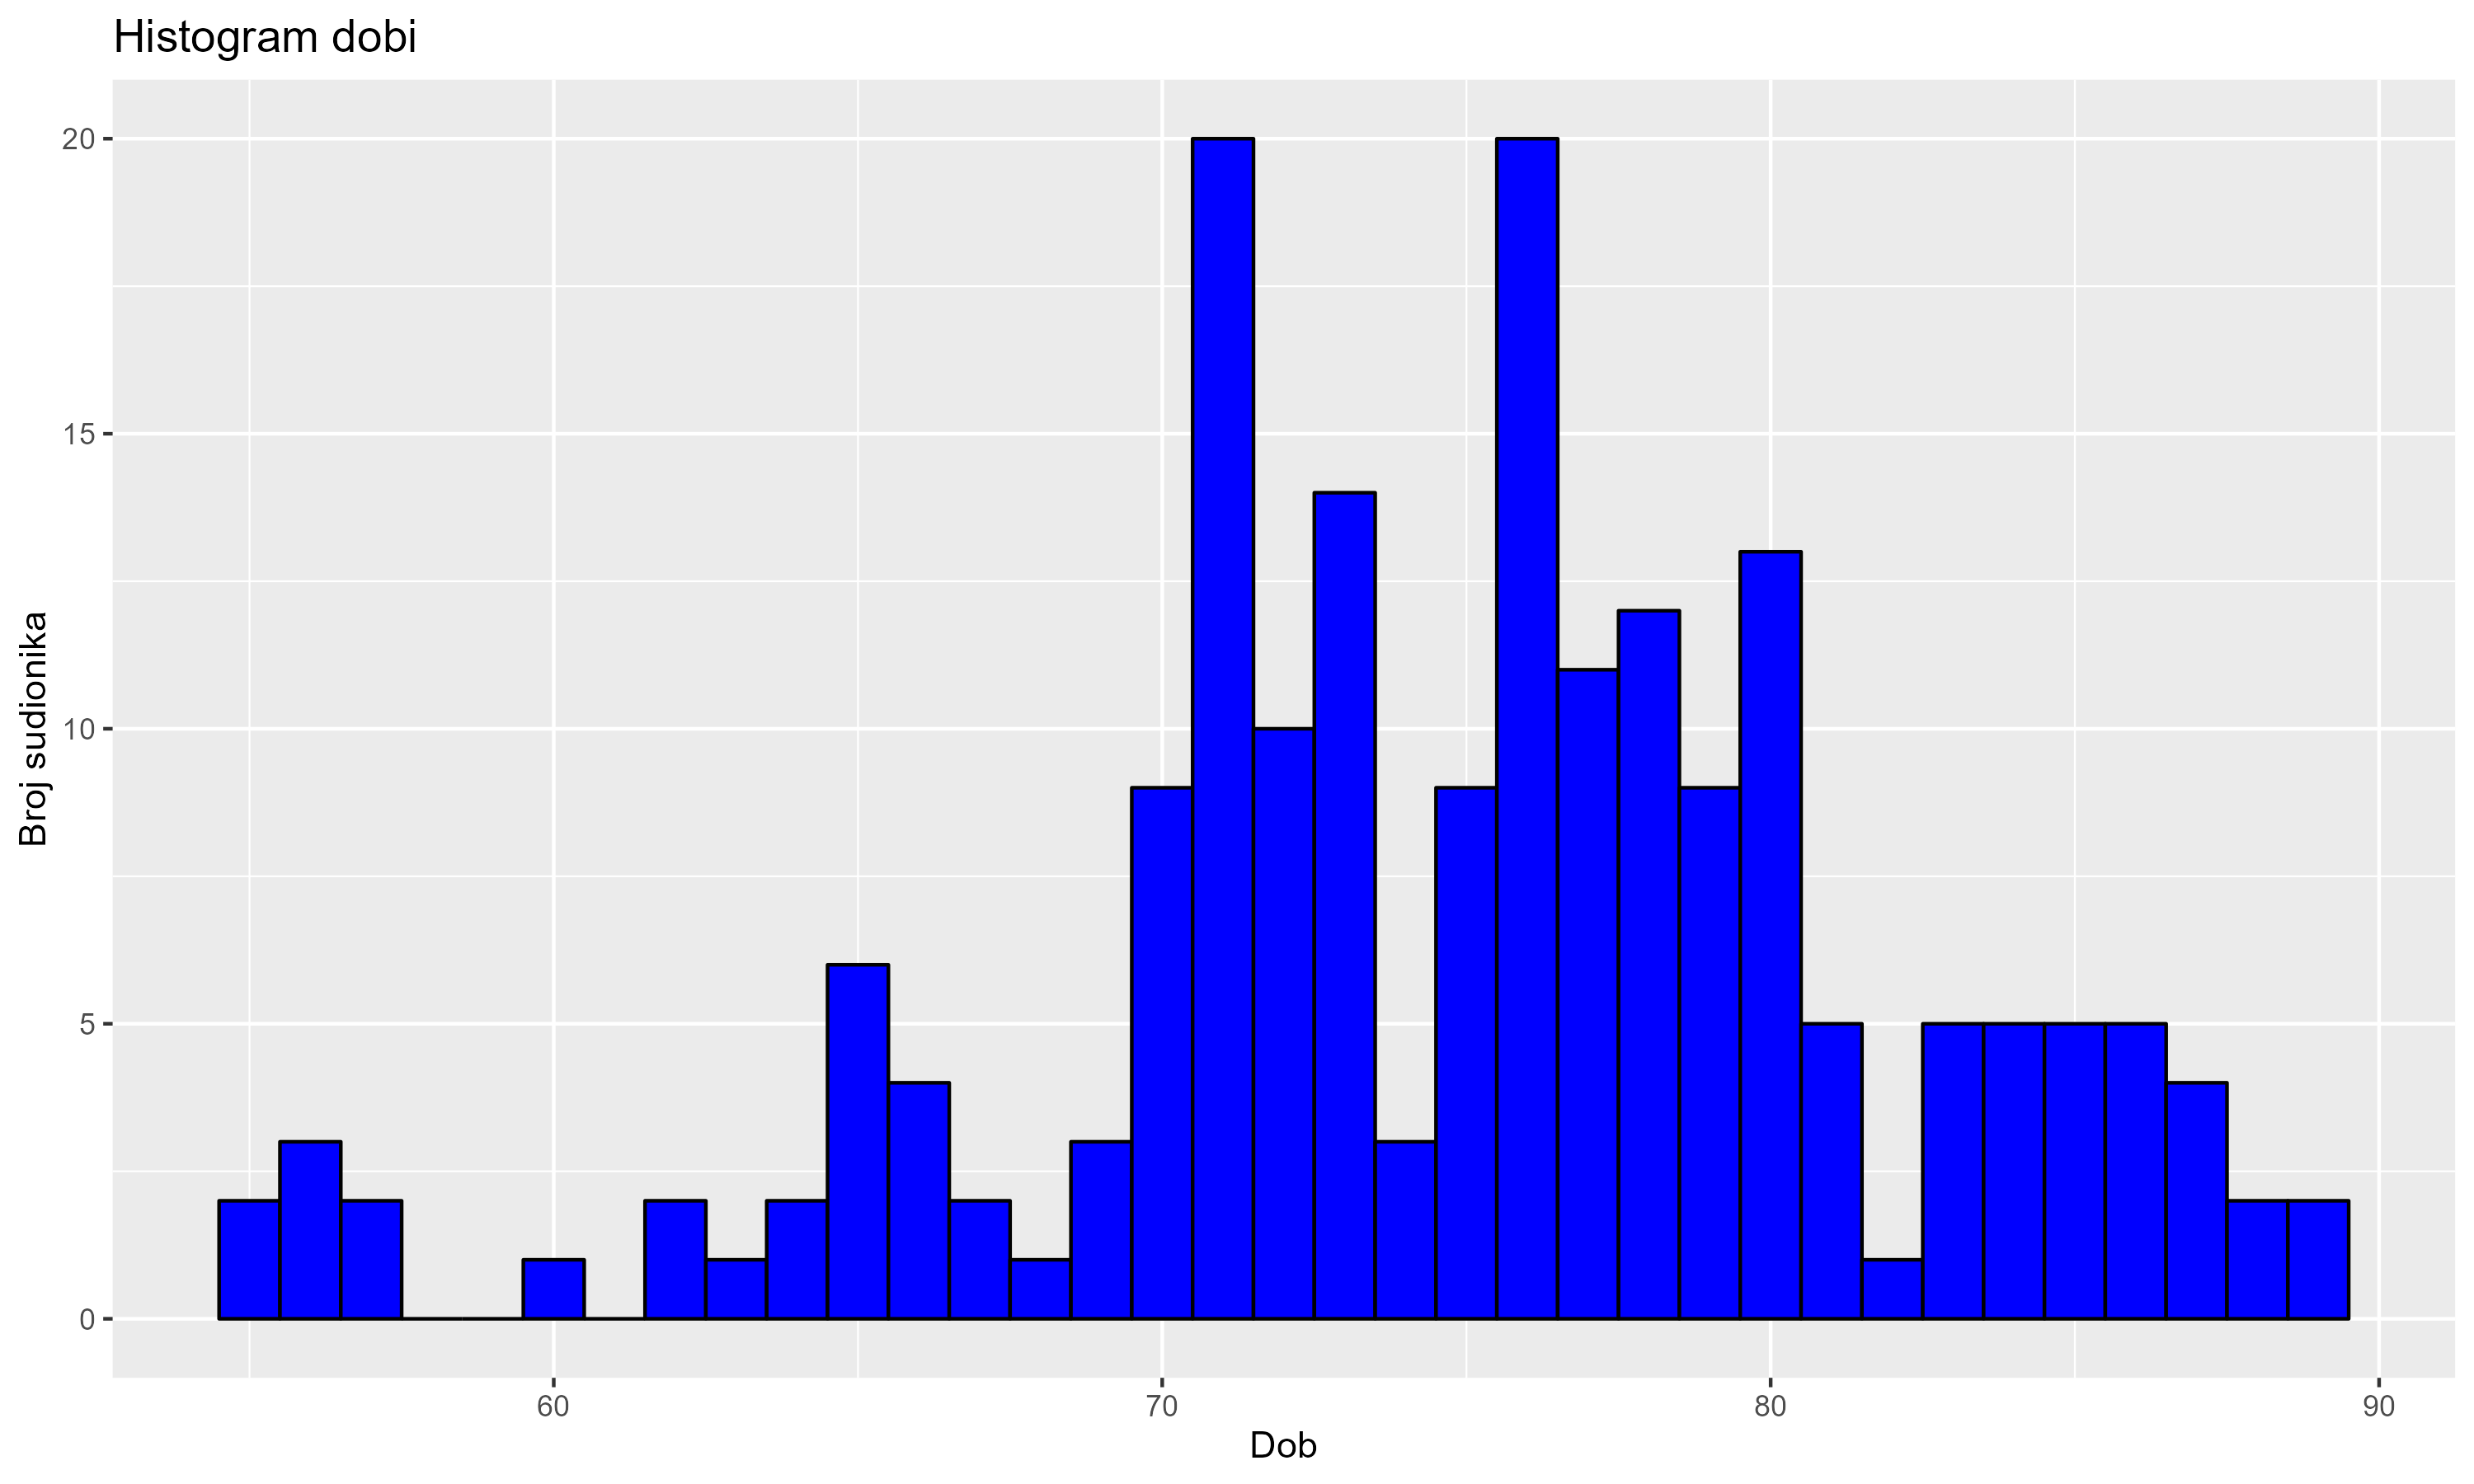
\includegraphics[width=0.8\textwidth]{Figures/histogram_dobi.png}
	\caption{Raspodjela sudionika po dobi}
	\label{fig:dob}
\end{figure}


\section{Implementacija}
U ovom poglavlju ćemo detaljno opisati implementaciju različitih modela strojnog učenja za klasifikaciju Alzheimerove bolesti koristeći strukturne MRI slike u NIfTI formatu. Implementirali smo tri modela: Stablo odluke, Random Forest i Support Vector Machine. Podaci su dobiveni iz ADNI baze podataka i obuhvaćaju tri klase: AD (Alzheimerova bolest), MCI (blagi kognitivni poremećaj) i CN (kognitivno normalni). Koristit ćemo Python programski jezik i niz biblioteka koje podržavaju strojno učenje i obradu medicinskih slika.

\subsection{Učitavanje i priprema podataka}
Prvi korak je učitavanje biblioteka, podataka iz CSV datoteke i priprema NIfTI slika za analizu.

\begin{lstlisting}[language=Python, caption={Učitavanje Python biblioteka}]
	import os
	import numpy as np
	import pandas as pd
	from nilearn import image
	from sklearn.model_selection import cross_val_score, cross_val_predict
	from sklearn.tree import DecisionTreeClassifier
	from sklearn.ensemble import RandomForestClassifier
	from sklearn.svm import SVC
	from sklearn.metrics import classification_report, confusion_matrix
	from sklearn.preprocessing import LabelEncoder
	from skimage.transform import resize
	from imblearn.over_sampling import RandomOverSampler
\end{lstlisting}

\noindent \textbf{Objašnjenje biblioteka:}
\begin{itemize}
	\item \texttt{os}: Biblioteka za rad s datotečnim sustavom.
	\item \texttt{numpy}: Biblioteka za rad s numeričkim podacima.
	\item \texttt{pandas}: Biblioteka za manipulaciju i analizu podataka u tabularnom obliku (.csv).
	\item \texttt{nilearn}: Biblioteka za neuroznanstvene analize, posebno rad s NIfTI slikama.
	\item \texttt{sklearn}: Biblioteka za strojno učenje koja sadrži alate za predprocesiranje, modeliranje i evaluaciju.
	\item \texttt{skimage}: Biblioteka za obradu slika.
	\item \texttt{imblearn}: Biblioteka za rad s neuravnoteženim podacima, uključujući tehniku oversamplinga.
\end{itemize}

\subsection{Učitavanje CSV podataka i generiranje putanja do NIfTI datoteka}

\begin{lstlisting}[language=Python, caption={Učitavanje podataka i generiranje putanja}]
	# Ucitavanje CSV podataka
	csv_path = "./ADNI1_Baseline_3T_3_20_2024.csv"
	source_path = "./ADNI_data"
	image_paths = get_paths(csv_path, source_path)
\end{lstlisting}

\noindent \textbf{Objašnjenje:}
\begin{itemize}
	\item \texttt{pd.read\_csv()}: Učitava podatke iz CSV datoteke.
	\item \texttt{get\_paths()}: Generira putanje do NIfTI datoteka na osnovu informacija iz CSV datoteke.
\end{itemize}

\subsection{Metoda \texttt{get\_paths()}}

Metoda \texttt{get\_paths()} koristi se za generiranje putanja do NIfTI datoteka na osnovu informacija iz CSV datoteke. Ova metoda čita CSV datoteku, obrađuje relevantne informacije i stvara popis putanja do NIfTI datoteka koje se koriste za daljnju analizu.

\begin{lstlisting}[language=Python, caption={Metoda get\_paths}]
	def get_paths(csv_path, source_path):
	csv = pd.read_csv(csv_path)
	filepaths = []
	for key, value in csv.iterrows():
	if value['Description'].endswith("Scaled"):
	modality_description = value['Description'].replace(';', '_').replace(' ', '_')
	acq_date = datetime.strptime(value['Acq Date'], '%m/%d/%Y').strftime('%Y-%m-%d')
	subject_path = os.path.join(source_path, value['Subject'], modality_description, acq_date, value['Image Data ID'])
	if os.path.exists(subject_path):
	with os.scandir(subject_path) as entries:
	file_name = next(entries).name
	smri_path = os.path.join(subject_path, file_name)
	filepaths.append(smri_path)
	return filepaths
\end{lstlisting}

\noindent \textbf{Objašnjenje:}
\begin{itemize}
	\item \texttt{pd.read\_csv()}: Učitava podatke iz CSV datoteke.
	\item \texttt{replace(';', '\_').replace(' ', '\_')}: Zamjenjuje znakove u opisu modaliteta kako bi bili prikladni za korištenje u putanjama.
	\item \texttt{datetime.strptime()}: Pretvara datum u odgovarajući format.
	\item \texttt{os.path.join()}: Stvara putanju do datoteke koristeći informacije iz CSV datoteke.
	\item \texttt{os.scandir()}: Iterira kroz direktorij i dohvaća ime prve datoteke.
	\item \texttt{filepaths.append(smri\_path)}: Dodaje putanju do fMRI datoteke u popis putanja.
\end{itemize}

\subsection{Učitavanje i promjena veličine NIfTI slika}

\begin{lstlisting}[language=Python, caption={Učitavanje i promjena veličine NIfTI slika}]
	fixed_shape = (64, 64, 64)
	images = []
	for path in image_paths:
	try:
	if os.path.exists(path):
	img = image.load_img(path)
	img_resized = resize(img.get_fdata(), fixed_shape, anti_aliasing=True)
	images.append(img_resized)
	except Exception as e:
	print(f"Error loading image {path}: {e}")
	
	# Konverzija slika u nizove
	X = np.array(images)
\end{lstlisting}

\noindent \textbf{Objašnjenje:}
\begin{itemize}
	\item \texttt{image.load\_img()}: Učitava NIfTI sliku.
	\item \texttt{resize()}: Mijenja veličinu slike na zadanu dimenziju \texttt{64x64x64}.
	\item \texttt{np.array()}: Konvertira listu slika u Numpy niz.
\end{itemize}

\subsection{Predprocesiranje podataka}

\begin{lstlisting}[language=Python, caption={Predprocesiranje podataka}]
	data = pd.read_csv(csv_path)
	labels = data['Group'][data['Description'].str.endswith("Scaled")]
	
	# Label encoding (konverzija labela u integer vrijednosti)
	label_encoder = LabelEncoder()
	y = label_encoder.fit_transform(labels)
	print("Class 0:", label_encoder.classes_[0])
	print("Class 1:", label_encoder.classes_[1])
	print("Class 2:", label_encoder.classes_[2])
	
	# Promjena oblika podataka
	X_flat = X.reshape(X.shape[0], -1)
	
	# Oversampling
	oversampler = RandomOverSampler()
	X_resampled, y_resampled = oversampler.fit_resample(X_flat, y)
\end{lstlisting}

\noindent \textbf{Objašnjenje:}
\begin{itemize}
	\item \texttt{LabelEncoder}: Konvertira kategorijske etikete u numeričke vrijednosti.
	\item \texttt{reshape()}: Mijenja oblik matrice slika u vektor.
	\item \texttt{RandomOverSampler}: Tehnika za balansiranje klasa povećavanjem broja uzoraka manjinskih klasa.
\end{itemize}

\subsection{Trening i evaluacija modela}

Za svaki model definiramo klasu \texttt{ModelTrainer} koja će olakšati proces treniranja i evaluacije.

\begin{lstlisting}[language=Python, caption={Klasa ModelTrainer}]
	class ModelTrainer:
	def __init__(self, model, model_name):
	self.model = model
	self.model_name = model_name
	self.y_pred = None
	
	def evaluate_model(self, X, y):
	print(f"\nEvaluating {self.model_name}...")
	scores = cross_val_score(self.model, X, y, cv=5)
	print(f"{self.model_name} cross-validation scores:", scores)
	print(f"Mean {self.model_name} cross-validation score:", scores.mean())
	return scores
	
	def train_and_predict(self, X, y):
	self.model.fit(X, y)
	self.y_pred = cross_val_predict(self.model, X, y, cv=5)
	print(f"\n{self.model_name} classification report:")
	print(classification_report(y, self.y_pred, zero_division=1))
	print(f"\n{self.model_name} confusion matrix: ")
	print(confusion_matrix(y, self.y_pred))
	return self.y_pred
\end{lstlisting}

\noindent \textbf{Objašnjenje:}
\begin{itemize}
	\item \texttt{cross\_val\_score()}: Evaluira model koristeći k-fold tehniku \textbf{unakrsne validacije}. U našoj implementaciji koristili smo k-fold unakrsnu validaciju s k=5. To znači da je cijeli skup podataka podijeljen na 5 podskupova. Model je treniran na 4 podskupa, dok je 5. podskup korišten za testiranje. Ovaj proces ponovljen je 5 puta, svaki put koristeći drugi podskup za testiranje. Konačne performanse modela izračunate su kao prosjek performansi na svih 5 iteracija.
	\item \texttt{fit()}: Treniranje modela na podacima.
	\item \texttt{cross\_val\_predict()}: Generira predikcije koristeći cross-validation.
	\item \texttt{classification\_report()}: Prikazuje detaljan izvještaj klasifikacije uključujući preciznost, odziv i F1 mjeru.
	\item \texttt{confusion\_matrix()}: Prikazuje matricu konfuzije koja prikazuje točne i netočne klasifikacije.
\end{itemize}


\subsection{Stablo odluke}

\begin{lstlisting}[language=Python, caption={Trening i evaluacija Stablo odluke modela}]
	# Trening i evaluacija Stablo odluke modela
	decision_tree = DecisionTreeClassifier()
	dt_trainer = ModelTrainer(decision_tree, "Decision Tree")
	dt_trainer.evaluate_model(X_resampled, y_resampled)
	y_pred_dt = dt_trainer.train_and_predict(X_resampled, y_resampled)
\end{lstlisting}

\noindent \textbf{Objašnjenje:}
\begin{itemize}
	\item \texttt{DecisionTreeClassifier}: Implementira algoritam stabla odlučivanja.
\end{itemize}

\subsection{Random Forest}

\begin{lstlisting}[language=Python, caption={Trening i evaluacija Random Forest modela}]
	# Trening i evaluacija Random Forest modela
	random_forest = RandomForestClassifier(n_estimators=100, random_state=42)
	rf_trainer = ModelTrainer(random_forest, "Random Forest")
	rf_trainer.evaluate_model(X_resampled, y_resampled)
	y_pred_rf = rf_trainer.train_and_predict(X_resampled, y_resampled)
\end{lstlisting}

\noindent \textbf{Objašnjenje:}
\begin{itemize}
	\item \texttt{RandomForestClassifier}: Implementira algoritam Random Forest koristeći 100 stabala (\texttt{n\_estimators=100}).
\end{itemize}

\subsection{Support Vector Machine}

\begin{lstlisting}[language=Python, caption={Trening i evaluacija SVM modela}]
	# Trening i evaluacija SVM modela
	svm = SVC(kernel='linear', random_state=42)
	svm_trainer = ModelTrainer(svm, "Support Vector Machine")
	svm_trainer.evaluate_model(X_resampled, y_resampled)
	y_pred_svm = svm_trainer.train_and_predict(X_resampled, y_resampled)
\end{lstlisting}

\noindent \textbf{Objašnjenje:}
\begin{itemize}
	\item \texttt{SVC}: Implementira Support Vector Machine s linearnom kernel funkcijom.
\end{itemize}


%-------------------------------------------------------------------------------
\chapter{Rezultati i rasprava}
\label{pog:rezultati_i_rasprava}

\section{Osnovni pojmovi}

Prije nego što predstavimo rezultate, važno je definirati ključne pojmove korištene u evaluaciji modela strojnog učenja.

\subsection{Točnost (Accuracy)}

Točnost je omjer točnih predikcija i ukupnog broja predikcija. To je jednostavna metrika koja pokazuje koliko je model precizan u svojim predikcijama:
\begin{equation}
	\text{Accuracy} = \frac{\text{Broj točnih predikcija}}{\text{Ukupan broj predikcija}}
\end{equation}

\subsection{Matrica zabune (Confusion Matrix)}

Matrica zabune je tablica koja prikazuje performanse modela klasifikacije na skupu testnih podataka za koje su poznate stvarne vrijednosti. Ona prikazuje broj točnih i netočnih predikcija za svaku klasu. Tipična matrica zabune \ref{tab:conf_matrix} izgleda ovako:

\begin{table}[h]
	\centering
	\begin{tabular}{c|c|c|c}
		& \textbf{Predikcija: Klasa 0} & \textbf{Predikcija: Klasa 1} & \textbf{Predikcija: Klasa 2} \\ \hline
		\textbf{Stvarna Klasa 0} & \cellcolor{green!25} & & \\ \hline
		\textbf{Stvarna Klasa 1} & & \cellcolor{green!25} & \\ \hline
		\textbf{Stvarna Klasa 2} & & & \cellcolor{green!25} \\ 
	\end{tabular}
	\caption{Primjer matrice konfuzije}
	\label{tab:conf_matrix}
\end{table}

\subsection{Preciznost (Precision), odziv (Recall) i F1-mjera (F1-score)}

\begin{itemize}
	\item \textbf{Preciznost (Precision)} je omjer točnih pozitivnih predikcija i ukupnog broja pozitivnih predikcija \cite{medium_confusion_matrix}:
	\begin{equation}
		\text{Precision} = \frac{\text{Točno pozitivni}}{\text{Točno pozitivni + Netočno pozitivni}}
	\end{equation}
	\item \textbf{Odziv (Recall)} je omjer točnih pozitivnih predikcija i ukupnog broja stvarnih pozitivnih slučajeva \cite{medium_confusion_matrix}:
	\begin{equation}
		\text{Recall} = \frac{\text{Točno pozitivni}}{\text{Točno pozitivni + Netočno negativni}}
	\end{equation}
	\item \textbf{F1-mjera (F1-score)} je harmonijska sredina preciznosti i odziva \cite{towardsdatascience_confusion_matrix}:
	\begin{equation}
		\text{F1-score} = 2 \times \frac{\text{Precision} \times \text{Recall}}{\text{Precision + Recall}}
	\end{equation}
\end{itemize}


\subsection{Težinski uprosječene mjere (Weighted avg) i makro-usprosječene mjere (Macro avg)}

\textbf{Weighted avg} također izračunava metričku vrijednost (preciznost, odziv ili F1-score) za svaku klasu, ali uzima u obzir broj uzoraka u svakoj klasi prilikom izračunavanja prosjeka \cite{Mathew2023}. To znači da klase s više uzoraka imaju veću težinu u konačnom prosjeku. Na primjer, ako imamo tri klase s preciznostima od 0.71, 0.61 i 0.59 i brojem uzoraka od 92, 92 i 92, njihov weighted average bi bio:
\[ \text{Weighted Avg Precision} = \frac{(92 \times 0.71) + (92 \times 0.61) + (92 \times 0.59)}{276} = 0.64 \]

\textbf{Macro avg} izračunava metričku vrijednost (preciznost, odziv ili F1-score) za svaku klasu pojedinačno i zatim izračunava prosjek tih vrijednosti \cite{Mathew2023}. Svaka klasa ima jednaku težinu, bez obzira na broj uzoraka u toj klasi. Na primjer, ako imamo tri klase s preciznostima od 0.71, 0.61 i 0.59, njihov macro average bi bio:
\[ \text{Macro Avg Precision} = \frac{0.71 + 0.61 + 0.59}{3} = 0.64 \]


\section{Rezultati klasifikacije}

Kao što je prikazano u prethodnom poglavlju, implementirali smo tri različita modela za klasifikaciju Alzheimerove bolesti (AD), blagog kognitivnog poremećaja (MCI) i kognitivno normalnih (CN) subjekata koristeći strukturne MRI slike. Ovdje ćemo prikazati dobivene rezultate nakon unakrsne validacije za svaki model.

\noindent \textbf{Distribucija klasa:}
\begin{itemize}
	\item Class 0: AD
	\item Class 1: CN
	\item Class 2: MCI
\end{itemize}


\subsection{Stablo odluke}

Rezultati za DT model:

\begin{verbatim}
	Evaluating Decision Tree...
	
	Decision Tree cross-validation scores: [0.52380952 0.64285714 0.58536585 0.75609756 0.7804878 ]
	Mean Decision Tree cross-validation score: 0.6577235772357722
	
	Decision Tree classification report:
	precision    recall  f1-score   support
	
	0       0.69      0.88      0.78        69
	1       0.64      0.62      0.63        69
	2       0.69      0.52      0.60        69
	
	accuracy                           0.68       207
	
	macro avg       0.68      0.68      0.67       207
	
	weighted avg       0.68      0.68      0.67       207
\end{verbatim}

\begin{figure}[h]
	\centering
	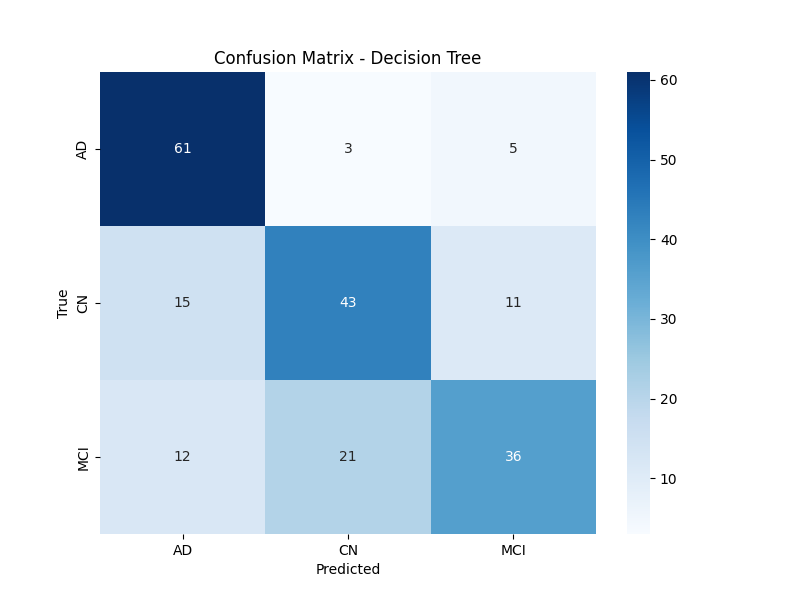
\includegraphics[width=0.7\textwidth]{Figures/matrix_dt_2.png}
	\caption{Confusion Matrix - Decision Tree}
	\label{fig:matrix_dt}
\end{figure}

\subsection{Slučajna šuma}

Rezultati za RF model:

\begin{verbatim}
	Evaluating Random Forest...
	
	Random Forest cross-validation scores: [0.5        0.5952381  0.70731707 0.80487805 0.75609756]
	Mean Random Forest cross-validation score: 0.6727061556329849
	
	Random Forest classification report:
	precision    recall  f1-score   support
	
	0       0.70      0.90      0.79        69
	1       0.63      0.65      0.64        69
	2       0.67      0.46      0.55        69
	
	accuracy                           0.67       207
	
	macro avg       0.67      0.67      0.66       207
	
	weighted avg       0.67      0.67      0.66       207
\end{verbatim}

\begin{figure}[h]
	\centering
	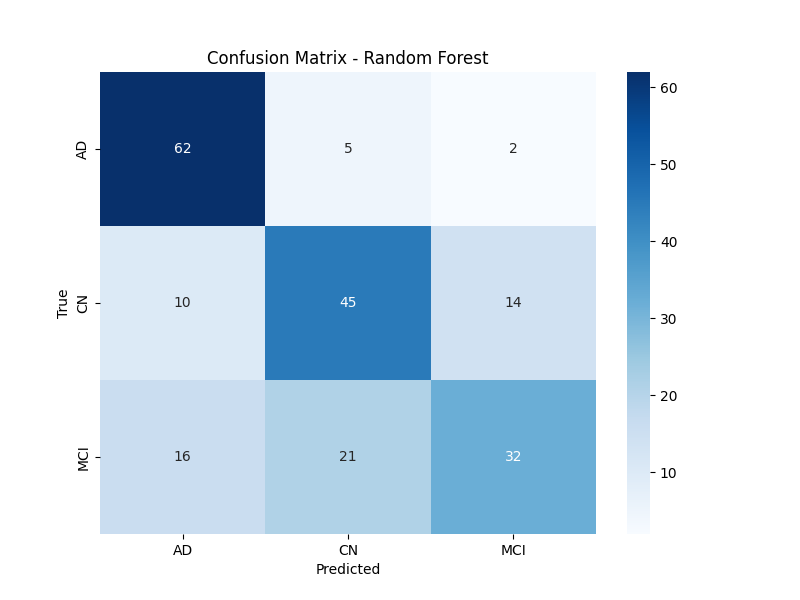
\includegraphics[width=0.7\textwidth]{Figures/matrix_rf_2.png}
	\caption{Confusion Matrix - Random Forest}
	\label{fig:matrix_rf}
\end{figure}

\subsection{Stroj potpornih vektora}

Rezultati za SVM model:

\begin{verbatim}
	Evaluating Support Vector Machine...
	
	Support Vector Machine cross-validation scores: [0.52380952 0.57142857 0.53658537 0.85365854 0.7804878 ]
	Mean Support Vector Machine cross-validation score: 0.6531939605110336
	
	Support Vector Machine classification report:
	precision    recall  f1-score   support
	
	0       0.73      0.91      0.81        69
	1       0.65      0.65      0.65        69
	2       0.62      0.46      0.53        69
	
	accuracy                           0.68       207
	
	macro avg       0.67      0.68      0.66       207
	
	weighted avg       0.67      0.68      0.66       207
\end{verbatim}

\begin{figure}[h]
	\centering
	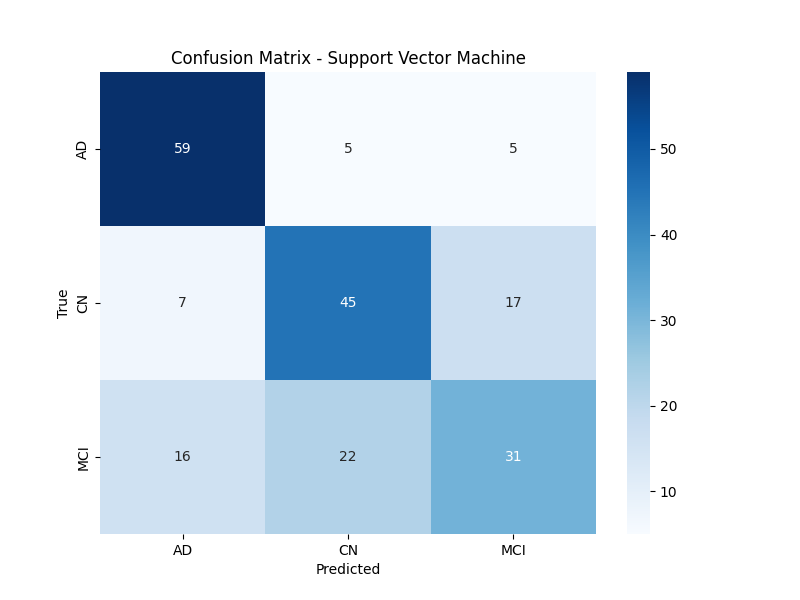
\includegraphics[width=0.7\textwidth]{Figures/matrix_svm_2.png}
	\caption{Confusion Matrix - Support Vector Machine}
	\label{fig:matrix_svm}
\end{figure}

\subsection{Usporedba rezultata}

Usporedba rezultata između modela prikazana je u tablici \ref{tab:classification_results}.

\begin{table}[h!]
	\centering
	\begin{tabularx}{\textwidth}{|X|X|X|X|}
		\hline
		& \textbf{Stablo odluke} & \textbf{Random Forest} & \textbf{Support Vector Machine} \\ \hline
		\textbf{Cross-validation scores} & [0.52380952, 0.64285714, 0.58536585, 0.75609756, 0.7804878] & [0.5, 0.5952381, 0.70731707, 0.80487805, 0.75609756] & [0.52380952, 0.57142857, 0.53658537, 0.85365854, 0.7804878] \\ \hline
		\textbf{Mean cross-validation score} & 0.6577 & 0.6727 & 0.6532 \\ \hline
		\textbf{Precision (Class 0: AD)} & 0.69 & 0.70 & 0.73 \\ \hline
		\textbf{Precision (Class 1: CN)} & 0.64 & 0.63 & 0.65 \\ \hline
		\textbf{Precision (Class 2: MCI)} & 0.69 & 0.67 & 0.62 \\ \hline
		\textbf{Recall (Class 0: AD)} & 0.88 & 0.90 & 0.91 \\ \hline
		\textbf{Recall (Class 1: CN)} & 0.62 & 0.65 & 0.65 \\ \hline
		\textbf{Recall (Class 2: MCI)} & 0.52 & 0.46 & 0.46 \\ \hline
		\textbf{F1-score (Class 0: AD)} & 0.78 & 0.79 & 0.81 \\ \hline
		\textbf{F1-score (Class 1: CN)} & 0.63 & 0.64 & 0.65 \\ \hline
		\textbf{F1-score (Class 2: MCI)} & 0.60 & 0.55 & 0.53 \\ \hline
		\textbf{Accuracy} & 0.68 & 0.67 & 0.68 \\ \hline
		\textbf{Macro avg precision} & 0.68 & 0.67 & 0.67 \\ \hline
		\textbf{Macro avg recall} & 0.68 & 0.67 & 0.68 \\ \hline
		\textbf{Macro avg F1-score} & 0.67 & 0.66 & 0.66 \\ \hline
		\textbf{Weighted avg precision} & 0.68 & 0.67 & 0.67 \\ \hline
		\textbf{Weighted avg recall} & 0.68 & 0.67 & 0.68 \\ \hline
		\textbf{Weighted avg F1-score} & 0.67 & 0.66 & 0.66 \\ \hline
	\end{tabularx}
	\caption{Usporedba rezultata klasifikacijskih modela}
	\label{tab:classification_results}
\end{table}

\begin{itemize}
	\item \textbf{Točnost (accuracy)}: Stablo odluke i SVM postižu točnost od 0.68, dok Random Forest postiže točnost od 0.67.
	\item \textbf{Precision i Recall}: SVM model ima najvišu preciznost i recall za klasu AD (Preciznost: 0.73, Recall: 0.91). Međutim, svi modeli imaju sličan rezultat.
    \item \textbf{Confusion Matrix}: Sve tri matrice konfuzije pokazuju da modeli imaju problema s ispravnim klasificiranjem MCI slučajeva, što može biti rezultat sličnosti MCI klasa s ostalim klasama, što otežava pravilno razlikovanje.
    \item \textbf{Cross-validation score}: Random Forest pokazuje najveću prosječnu točnost u rezultatima unakrsne validacije, što ukazuje na bolju generalizaciju u odnosu na druge modele.
    \item \textbf{Classification report}: Preciznost, recall i F1-score daju detaljan pregled performansi modela po klasama. Support Vector Machine ima najvišu vrijednost ovih metrika za većinu klasa.
\end{itemize}


\subsection{Usporedba s drugim istraživanjima}

U ovom dijelu analizirat ćemo rezultate našeg istraživanja u usporedbi s rezultatima iz nekoliko relevantnih radova koji su također koristili metode strojnog učenja za klasifikaciju Alzheimerove bolesti, blagog kognitivnog poremećaja i kognitivno normalnih subjekata.

U radu \cite{MultimodalRF} autori istražuju učinkovitost Random Forest modela za klasifikaciju Alzheimerove bolesti koristeći multimodalne MRI podatke iz TADPOLE dataset-a, koji je dio ADNI inicijative. Korištenjem strukturnih MRI, DTI i rs-fMRI podataka, autori su postigli točnost od 69.33\%. Makro prosječna preciznost bila je 69.33\%, dok je makro prosječan recall iznosio 40.94\%, a makro prosječan F1-score 51.48\%. Naši rezultati za Random Forest model pokazuju točnost od 67\%, s makro prosječnom preciznošću od 67\%, makro prosječnim recall-om od 67\% i makro prosječnim F1-score-om od 66\%. Ovi rezultati sugeriraju da naš model ima sličnu učinkovitost u klasifikaciji različitih stadija Alzheimerove bolesti, ali postoji prostor za poboljšanje u usporedbi s njihovim rezultatima.

U radu \cite{IRJET}, autori su pregledali različite algoritme strojnog učenja za klasifikaciju stadija Alzheimerove bolesti koristeći MRI podatke iz ADNI baze. Posebnu pažnju posvetili su Support Vector Machine (SVM) algoritmu. Rezultati koje su postigli pokazuju visoku točnost za različite parove klasa: EMCI vs. CN 93.8\%, LMCI vs. CN 95.8\%, AD vs. CN 95.8\% i LMCI vs. AD 91.7\%. Naš SVM model postigao je ukupnu točnost od 68\%, s makro prosječnom preciznošću od 67\%, makro prosječnim recall-om od 68\% i makro prosječnim F1-score-om od 66\%. Iako su naši rezultati niži u usporedbi s njihovim specifičnim točnostima za parove klasa, važno je napomenuti da su njihovi rezultati specifični za određene klasifikacije, dok naši rezultati predstavljaju ukupnu učinkovitost modela za sve klase.

U radu \cite{AnalysisPerformance}, autori su analizirali performanse različitih tehnika strojnog učenja, uključujući Random Forest, za otkrivanje i klasifikaciju Alzheimerove bolesti koristeći MRI podatke. Korištenje Random Forest modela u njihovoj studiji rezultiralo je točnošću od 69.33\%, makro prosječnom preciznošću od 69.33\%, makro prosječnim recall-om od 40.94\% i makro prosječnim F1-score-om od 51.48\%. U usporedbi s našim rezultatima, naš Random Forest model pokazuje točnost od 67\% i slične makro prosječne metrike (precision: 67\%, recall: 67\%, F1-score: 66\%). Ovi rezultati ukazuju na sličnu učinkovitost našeg modela u klasifikaciji Alzheimerove bolesti, ali postoji prostor za poboljšanje u usporedbi s njihovim rezultatima.

U radu \cite{asi}, istražena je klasifikacija Alzheimerove bolesti koristeći Stablo odluke, SVM i Ensemble modele. Njihovi rezultati pokazuju točnost Stablo odluke modela od 86.8\%, dok SVM i Ensemble modeli postižu točnost od 87.2\% i 86.3\% respektivno. Ovi rezultati ukazuju na visoku točnost koju je moguće postići korištenjem jednostavnijih modela uz pravilnu obradu podataka. Naš Stablo odluke model postigao je točnost od 68\%, s makro prosječnom preciznošću od 68\%, makro prosječnim recall-om od 68\% i makro prosječnim F1-score-om od 67\%. Ovi rezultati su niži u usporedbi s rezultatima iz literature, što sugerira da je moguće poboljšati naš model korištenjem boljih tehnika obrade podataka ili optimizacije modela.
%--- ZAKLJUČAK / CONCLUSION ----------------------------------------------------
\chapter{Zaključak}
\label{pog:zakljucak}
U ovom radu smo istražili primjenu modela strojnog učenja za klasifikaciju Alzheimerove bolesti koristeći strukturne MRI slike iz ADNI baze podataka. Fokusirali smo se na implementaciju i evaluaciju triju različitih modela: Stablo odluke, Slučajna šuma i SVM. Cilj je bio usporediti njihove performanse i utvrditi koji model pruža najbolje rezultate u klasifikaciji Alzheimerove bolesti, blagih kognitivnih poremećaja i kognitivno normalnih subjekata.

Korištenjem dostupnih podataka, najprije smo izvršili pripremu podataka te njihovu prilagodbu u standardizirani format pogodniji za ulaz u modele strojnog učenja. Nadalje, koristili smo metode poput prekomjernog uzorkovanja kako bismo se nosili s problemom neravnoteže klasa, što je čest problem u medicinskim istraživanjima. Oversampling tehnika umjetno generira dodatne uzorke za klase s manjim brojem podataka, što nam je pomoglo u boljem balansiranju dataset-a.

Usporedba naših rezultata s relevantnim radovima iz literature pokazuje da su naši modeli konkurentni, ali postoje područja za poboljšanje.

Ovi rezultati ukazuju na nekoliko važnih zaključaka. 
Prvo, svi modeli pokazali su slične rezultate u klasifikaciji Alzheimerove bolesti, blagih kognitivnih poremećaja i kognitivno normalnih subjekata. SVM model pokazao je najvišu preciznost i recall za klasu AD, dok su Stablo odluke i Slučajna šuma pokazali prednosti u drugim metrikama.
Drugo, klasifikacija MCI slučajeva predstavljala je izazov za sve modele, što sugerira potrebu za daljnjim istraživanjem u ovoj domeni, možda kroz korištenje dodatnih značajki ili kombinaciju različitih modela.
Treće, iako su naši modeli konkurentni, usporedba s radovima iz literature pokazuje da postoji prostor za poboljšanje, posebno kroz optimizaciju modela i poboljšanje metoda obrade podataka. Također, korištenje oversamplinga može utjecati na rezultate, stoga je potrebno dodatno istražiti efekte ove tehnike na performanse modela.

Što se tiče budućeg rada, bilo bi dobro usmjeriti se na istraživanje naprednijih tehnika obrade podataka i značajki, te korištenje metoda koje kombiniraju prednosti različitih modela. Također, korištenje dubokog učenja može pružiti dodatne prednosti, posebno u prepoznavanju složenih uzoraka u MRI slikama.


%--- LITERATURA / REFERENCES ---------------------------------------------------

% Literatura se automatski generira iz zadane .bib datoteke / References are automatically generated from the supplied .bib file
% Upiši ime BibTeX datoteke bez .bib nastavka / Enter the name of the BibTeX file without .bib extension
\bibliography{literatura}



%--- SAŽETAK / ABSTRACT --------------------------------------------------------

% Sažetak na hrvatskom
\begin{sazetak}
	Ovaj rad istražuje primjenu strojnog učenja za klasifikaciju Alzheimerove bolesti koristeći strukturne MRI slike iz ADNI baze podataka. Implementirani su modeli stabla odluke, nasumične šume i stroja potpornih vektora (SVM). Model nasumične šume postiže točnost od 67\%, dok SVM postiže 65\%, a stablo odluke 68\%. Usporedba s relevantnim radovima iz literature pokazuje da naši modeli ostvaruju konkurentne rezultate, ali postoji prostor za poboljšanje, posebno u klasifikaciji slučajeva s blagim kognitivnim oštećenjem.
\end{sazetak}

\begin{kljucnerijeci}
	Strojno učenje; Alzheimerova bolest; Klasifikacija; Stablo odluke; Slučajna šuma; Stroj potpornih vektora; MRI; strukturni MRI
\end{kljucnerijeci}

% Abstract in English
\begin{abstract}
	This paper explores the application of machine learning for the classification of Alzheimer's disease using structural MRI images from the ADNI database. Implemented models include Decision Tree, Random Forest, and Support Vector Machine (SVM). The Random Forest model achieves an accuracy of 67\%, while SVM achieves 65\% and Decision Tree achieves 68\%. The comparison with relevant literature indicates that our models achieve competitive results, though there is room for improvement, particularly in classifying mild cognitive impairment.
\end{abstract}

\begin{keywords}
	machine learning; Alzheimer's disease; classification; Decision Tree; Random Forest; Support Vector Machine; MRI; structural MRI
\end{keywords}


%--- PRIVITCI / APPENDIX -------------------------------------------------------

% Sva poglavlja koja slijede će biti označena slovom i riječi privitak / All following chapters will be denoted with an appendix and a letter
\backmatter


\end{document}
